\documentclass[11pt,a4paper,oneside]{book}
\usepackage{fontspec}
\usepackage[top=2.5cm, bottom=2.5cm, left=2.5cm, right=2.5cm]{geometry}
\usepackage[utf8]{inputenc}
\usepackage[T1]{fontenc}
\usepackage[francais]{babel}
\usepackage{color}
\usepackage[table]{xcolor} % couleur dans un tableau
\usepackage{multirow} % fusion des lignes d'un tableau
\usepackage{tabularx}
\usepackage{pdflscape}
\usepackage{titlesec} % formater les titres
\usepackage[Glenn]{fncychap} % autre format titre
\usepackage{graphicx} % pour les images
\usepackage{chngcntr} % package pour changer la numérotation des figures

\graphicspath{ {./image/} } % chemin pour les images
 
\counterwithout{figure}{chapter}
\counterwithout{table}{chapter}

% ceci est un commentaire
\author{Hugo CELDRAN}
\title{Vieille et Recherche}
\title{Expert Cloud, Sécurité et Infrastructure}
\date{Ynov 2022}

\setmainfont{Calibri-Regular.ttf}[Path=./calibri/,
BoldFont       = Calibri-Bold.TTF,
BoldItalicFont = Calibri-Bold-Italic.ttf,
ItalicFont     = Calibri-Italic.ttf]

\renewcommand{\baselinestretch}{1.5} % interligne 1,5


\begin{document}

\maketitle
\tableofcontents


\chapter{Introduction}
% mettre eventuellement une citation dans l'intro pour montrer que c est un marche en essort comme ca ajout en plus dans la biblio

Dans le cadre de mon alternance, j'ai pris la décision de changer d'entreprise pour réaliser mon master.
En effet, ce choix était motivé par la volonté de découvrir un nouveau métier et les nouvelles missions qui l'accompagnent. \\

J'ai découvert alors le métier d'administrateur système dans une culture DevOps.
Le DevOps est un mouvement en ingénierie informatique et une pratique technique qui veut unifier le développement logiciel (Dev) et l'administration des infrastructures informatiques (Ops).
Le problème avec cette approche c'est qu'il n'y a pas d'aspect sécurité des systèmes et des logiciels, donc vous aviez des processus de développement et de déploiement confié à une équipe et à la phase finale une autre équipe gérée la sécurité.
Cela n'était pas gênant à une époque car les déploiement applicatifs ne se faisaient pas aussi régulièrement qu'aujourd'hui.
Par exemple, où je travaille, nous faisons environ cinq déploiement par jour, alors imaginons nous des grandes entreprises qui travaillent selon cette culture : Google, Netflix. Le nombre de déploiement est énorme alors ne pas inclure de sécurité dedans serait une erreur. \\

En effet dans le cadre de travail collaboratif du modèle DevOps, la sécurité est une responsabilité partagée, intégrée du début à la fin. Cette notion est si importante qu'elle a donné naissance à l'expression « DevSecOps » pour souligner la nécessité d'intégrer la sécurité aux projets DevOps. \\

C'est donc dans cette démarche que l'on peut se poser la problématique suivante : En quoi le DevSecOps contribue t il à améliorer l'infrastructure et son déploiement ? \\

Cette vieille a donc une importance dans mon projet professionnel et mon quotidien. \\

Nous verrons dans un premier la démarche méthodologique afin d'expliquer le procédé de l'élaboration de mon plan de veille, puis dans un second temps la présentation des résultats obtenues en trois axes : veille concurrentielle, technique / technologique et commerciale.


\chapter{Démarche méthodologique}

Dans cette partie, nous verrons comment j'ai procédé à l'élaboration de mon plan de veille, puis des mots clefs que j'ai pu utiliser selon mon sujet du DevSecOps ainsi que le tableau des ressources immobilisées.

\section{Élaboration du plan de veille}

Dans cette section, nous allons voir en 5 points ce qui m'a permit de réaliser mon plan de veille :
\begin{enumerate}
\item Identifier mon besoin ainsi que définir le périmètre qui en découle,
\item Collecter les informations qui m'intéressent,
\item Qualifier afin de savoir quelles informations je compte conserver,
\item Organiser pour savoir si les informations collecter sont pertinente,
\item Partager et utiliser afin de ne pas être seul à me servir de cette veille.
\end{enumerate}


\subsection{Définir le périmètre}

Mon sujet sur le DevSecOps est venu naturellement pour répondre à un besoin quotidien, mon métier.
En effet, cette veille me permet de me tenir au courant de toutes les mises à jours qui peuvent sortir ou encore me tenir au courant des différentes failles de sécurité qu'il peut exister pour m'en prémunir. \\

Cette veille est utile dans mon métier d'aujourd'hui mais ne correspond pas forcément à d'autres besoins à d'autres postes ou encore dans une entreprise différente. \\

Il a fallu que je définisse un périmètre afin d'être efficace et efficient. \\

Le périmètre peut être dans les sujets cherchés ou dans les ressources abordées.
Cela permet de ne pas perdre son temps sur internet en s'écartant du sujet et des recherches que l'on nous voulons faire. 
Les recherches sont souvent en anglais, tous les sites officiels des distributeurs des logiciels et donc les documentations le sont, et en français pour des articles détaillés sur les LinuxMagazine en général. \\

Je fais ma veille une à deux heures par jour en jours ouvrés.

\subsection{Collecter}

Pour collecter les informations de veille, j'ai utilisé un flux RSS.
Un flux RSS permet de récupérer sous format xml une information de mise à jour d'un site internet. Cela permet donc de surveiller plusieurs sources internet de façon automatiser et d'un seul et même endroit, notre outil choisi de flux RSS. \\

Pour moi, la mise en place de cet outil était pertinent, car nous devons faire attention aux mise à jours des plusieurs micro logiciels dont on se sert dans l'entreprise. Cela devient vite chronophage si l'information ne vient pas à nous. \\

Cela permet aussi d'éviter de consulter énormément de sites pour avoir les dernières informations qui sortent.

\subsection{Qualifier}

Une fois que l'information est venue jusqu'à nous, il faut à présent la qualifier, cela signifie que nous devons la classer.
Par exemple :
\begin{itemize}
\item Si une nouvelle technologie arrive bientôt, nous voudrons surveiller son évolution pour la tester et pourquoi pas la mettre en place à l'avenir,
\item Si par contre c'est une information d'une nouvelle mise à jour qui corrige un problème de  sécurité sur un logiciel il faudra rapidement le mettre en place.
\end{itemize}
Cette étape me permet de voir si les flux RSS reçus sont pertinents, car certains flux peuvent devenir obsolète (le logiciel suivi n'est plus utilisé) ou plus pertinent, je me suis abonné à un site qui ne publie pas que des articles sur mon domaine. \\
Dans certains cas, il faudra supprimer la source et d'entre cas réadapter le flux reçu.

\subsection{Organiser}

Une fois l'information qualifié, il faudra l'organiser, c'est à dire la prioriser en fonction de là où provient l'information. \\

Par exemple, si une nouvelle mise à jour d'un logiciel est sorti comme cela vient des sources officielles du concepteur je sais que je dois la prioriser en premier par rapport à une veille radar avec Twitter ou beaucoup d'informations superflux peuvent remonter. \\

Ce travail peut également se faire en configurant son flux dans des catégories, mais si un site est plus général, comme par exemple ma veille radar que je fais sur Twitter, on pourra le faire après avoir fait la qualification.
En effet, cela permettra de vérifier les sources est donc de déterminer si l'information est fiable et utilisable par la suite.

\subsection{Partager et utiliser}

J'ai choisi pour faire ma veille un outil de flux RSS (Tiny Tiny RSS) que l'on peut soi-même héberger.
On peut donc créer plusieurs utilisateurs qui interviendront sur la veille, mettre des catégories communes. \\

L'accès est fait grâce à une page internet, où l'on doit ensuite rentrer son nom d'utilisateur et son mot de passe. Mais cela reste sécurisé et seulement exploitable par les membres de l'entreprise. \\

\newpage

\section{Listes des mots clés}

Ces mots clés sont les mots principaux que j'utilise pour ma veille radar. \\

\begin{figure}[h]
\begin{tabularx}{14cm}{|X|}
\hline
\rowcolor{gray!30} Mots clefs \\
\hline
DevOps \\
DevSecOps \\
Linux \\
Terraform \\
Hashicorps \\
Kubernetes \\
Containers \\
Docker \\
Azure \\
AWS \\
Cloud \\
CNCF \\
Cloud Native Interactive Landscape \\
Helm \\
Gitlab \\
Deployement \\
Automatization \\
CI \\
CD \\
Infrastructure as code \\
CVE \\
Common Vulnerabilities and Exposures \\
\hline
\end{tabularx}
\caption{Tableau des mots clefs}
\end{figure}


\newpage

\begin{landscape}

\section{Tableau des ressources immobilisées}

Nous allons voir dans le tableau suivant les ressources immobilisées dans mon outil de flux RSS, je ne présente que les principales et les plus pertinents que j'utilise pour cette veille. \\

\begin{figure}[h]
\begin{tabular}{|l|c|c|c|c|c|c|}
\hline
\rowcolor{gray!30} Nom de la source / d'outil & Type & Lien & Auteur & Fréquence de la veille & Mots Clés & Provenance \\
\hline
GitHub Notifications release & technique & Privé & Multiple & tous les jours & & Flux RSS \\
CVE (faille de sécurité) & technique & https://cve.report/ & CVE report & tous les jours & & Flux RSS \\
Linux Fr & multiple & https://linuxfr.org/ & Multiple & tous les jours & & Flux RSS \\
Twitter Search & concurrentiel & https://twitter.com & Multiple & tous les jours & DevOps, DevSecOps & Réseau social \\
Linux Magazine & technique / économique & & Multiple & toutes les deux semaines & & Magazine \\
KubeCon & multiple & & Multiple & 1 fois par an & & Conférence \\
Mixit & multiple & & Multiple & 1 fois par an & & Conférence \\
JDLL & multiple & & Multiple & 1 fois par an & & Conférence \\
\hline
\end{tabular}
\caption{Tableau des ressources immobilisés}
\end{figure}


% Rajouter dans ce tableau les conferences types KubeCon & Mixit & JDLL

\end{landscape}


\chapter{Corps du dossier}

Nous verrons dans ce chapitre mes résultats issus des 3 axes de veille concurrentielle, technique / technologique et commerciale. \\

Dans un premier temps, nous verrons ce qu'est le DevSecOps dans son ensemble, dans un deuxième temps nous nous intéresserons au marché de celui-ci, dans un troisième temps les ressources et dans un dernier temps les enjeux et controverses autour du sujet.

\section{Le DevSecOps}

Dans cette section, nous allons dans un premier temps définir le DevSecOps, dans un deuxième temps nous ferrons un peu l'historique de ce terme et de son évolution dans le temps puis dans un dernier temps l'importance de ce sujet dans la société actuelle et du monde de l'informatique.

\subsection{Définition}

Pour comprendre le DevSecOps (abréviation de development, security, and operations), il faut s'intéresser au DevOps. \\

Le DevOps est définit par le processus de développement logiciel et un changement de culture organisationnelle.
Le but est accélérer la livraison de logiciels de meilleure qualité tout en automatisant et faisant travailler en équipe les développeurs et les infrastructures qui avant, avançait de manière séparée. \\

Le DevOps se veut de répondre à des demandes, en croissance, des utilisateurs de logiciels qui souhaitent de nouvelles fonctionnalités fréquentes, innovantes et performantes et de manière ininterrompue en disponibilité. \\

Finalement, le DevSecOps représente la même chose, il n'est que l'évolution naturelle du DevOps en intégrant un aspect sécurité pendant ces processus de développement et déploiement. \\

D'ailleurs pour la suite du rapport, je pourrais utiliser l'un ou l'autre terme mais aujourd'hui il se rejoigne fortement, l'extension Sec sert vraiment à appuyer cette intégration de sécurité.

\begin{figure}[h]
\centering
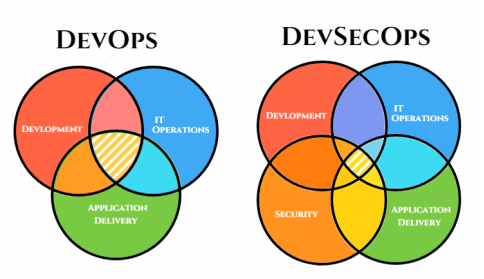
\includegraphics[scale=1]{devops-vs-devsecops}
\caption{Différence entre le DevOps et le DevSecOps}
\end{figure}

\subsection{Historique}

\begin{itemize}
\item 2001 Manifeste pour développement logiciel en mode Agile
\item 2007 Apparition du mot DevOps par Patrick Debois pendant une conférence
\item 2008 Google lance un groupe d'administrateur système en mode agile
\item 2010 DevOps Days en Belgique
\item 2012 IBM lance des outils DevOps
\item 2013 The Phoenix Project, une nouvelle fictive sur l'IT et le DevOps
\item 2014 Adoption du DevOps en accélération
\item 2018 "L'année du DevOps"
\end{itemize}

\subsection{Importance dans la société actuelle}

Le DevSecOps prend une importance dans notre société, car cette culture présente plusieurs avantages qui permettent de se concentrer sur de nouveaux sujets.
En effet, le fait d'automatiser certaines tâches permet de maximiser l'efficacité, cela permet également d'optimiser l'ensemble de l'activité tout en améliorant la rapidité et la stabilité du développement et du déploiement des logiciels.
L'intégration des méthodes de travail agile permet aussi de plus se concentrer sur l'humain et d'être dans une dynamique plus de recherche que de travail machine à répéter des tâches.

\newpage

\section{Le Marché}

Dans cette section, nous allons dans un premier temps voir l'État du marché du DevOps, dans un deuxième temps nous verrons les principaux acteurs puis dans un dernier temps les différentes parties prenantes.

\subsection{État du marché}

Le marché du DevOps était de 3,42 milliards Euro en 2018 à 10,31 milliards Euro d'ici 2023, à un taux de croissance annuel de 24,7 \% au cours de la période. \\

La demande de DevOps devrait être stimulée par plusieurs facteurs, tels que la réduction des coûts, la flexibilité, l'agilité et la livraison rapide des applications.

\subsection{Principaux acteurs}

La Cloud Native Computing Foundation (CNCF) est un projet de la Linux Foundation créé en 2015 pour faire progresser la technologie des conteneurs et orienter le secteur technologique vers son développement. \\

Parmi les membres fondateurs figurent Google, CoreOS, Mesosphere, Red Hat, Twitter, Huawei, Intel, Cisco, IBM, Docker, Univa et VMware. \\

D'autres entreprises qui n'ont pas fait parti de la création de cette fondation sont des acteurs importants dans le monde du DevSecOps. On peut par exemple citer Amazon et Azure.
Ces grandes entreprises influent aujourd'hui beaucoup ce marché en pleine expansion et en croissance.

\subsection{Parties prenantes}

Dev comprend toutes les personnes impliquées dans le développement de produits et services logiciels, y compris, mais sans s'y limiter : \\
\begin{itemize}
\item Architectes, représentants commerciaux, clients, propriétaires de produits, chefs de projet, testeurs et analystes, fournisseurs ... \\
\end{itemize}

Sec représente toutes les personnes impliqués dans la sécurité des produits et des services logiciels, y compris, mais sans s'y limiter : \\
\begin{itemize}
\item Professionnels de la sécurité de l'information, développeurs...
\end{itemize}

Ops inclut toutes les personnes impliquées dans la livraison et la gestion des produits et services logiciels, y compris, mais pas exclusivement, les personnes suivantes : \\
\begin{itemize}
\item Ingénieurs système, administrateurs système, ingénieurs d'exploitation informatique, ingénieurs de mise en production, administrateurs de bases de données (DBA), ingénieurs réseau, professionnels du support, vendeurs et fournisseurs tiers...
\end{itemize}

\newpage

\section{Les ressources}

Dans cette section, nous allons dans un premier temps les technologies identifiées, dans un second temps nous verrons les innovations et tendances dans le domaine.

\subsection{Technologies identifiées}

Il existe aujourd'hui de nombreuses technologies qui peuvent être utilisées pour le métier de DevSecOps.
Nous verrons les principaux outils utilisés au sein de l'entreprise où je travaille. \\
Un outil de version du code qui permet de suivre et d'avoir un historique et de travailler de manière collaborative : Git. \\
Pour l'intégration continue et le déploiement continu nous utilisons Gitlab. \\
Comme outil d'hébergement, nous sommes sur Azure Cloud et allons passer sur Aws (choix de la holding). \\
Dans les clusters, nous utilisons Kubernetes, qui est une plateforme d'orchestration de l'automatisation qui permet aux développeurs d'exécuter des applications conteneurisées sur des clusters Kubernetes faisant référence à un groupe de nœuds. Les développeurs exploitent Kubernetes pour automatiser des processus tels que la configuration des conteneurs, la mise à l'échelle, la mise en réseau, la sécurité, etc, afin de gagner en rapidité et en efficacité en production. \\
Nous combinons cette technologie avec Terraform qui permet de piloter l'ensemble des clusters. \\
Cela ne servirait pas plus à énumérer les autres qui restent encore nombreuses, ce qu'il faut comprendre c'est qu'il y a énormément de possibilités, de combinaisons et de synergies possibles.

\subsection{Innovations et tendances}

Pour les innovations et tendances, un site internet propose une énorme carte avec toutes les technologies disponibles. Ce site est proposé par CNCF. \\

\begin{figure}[h]
\centering
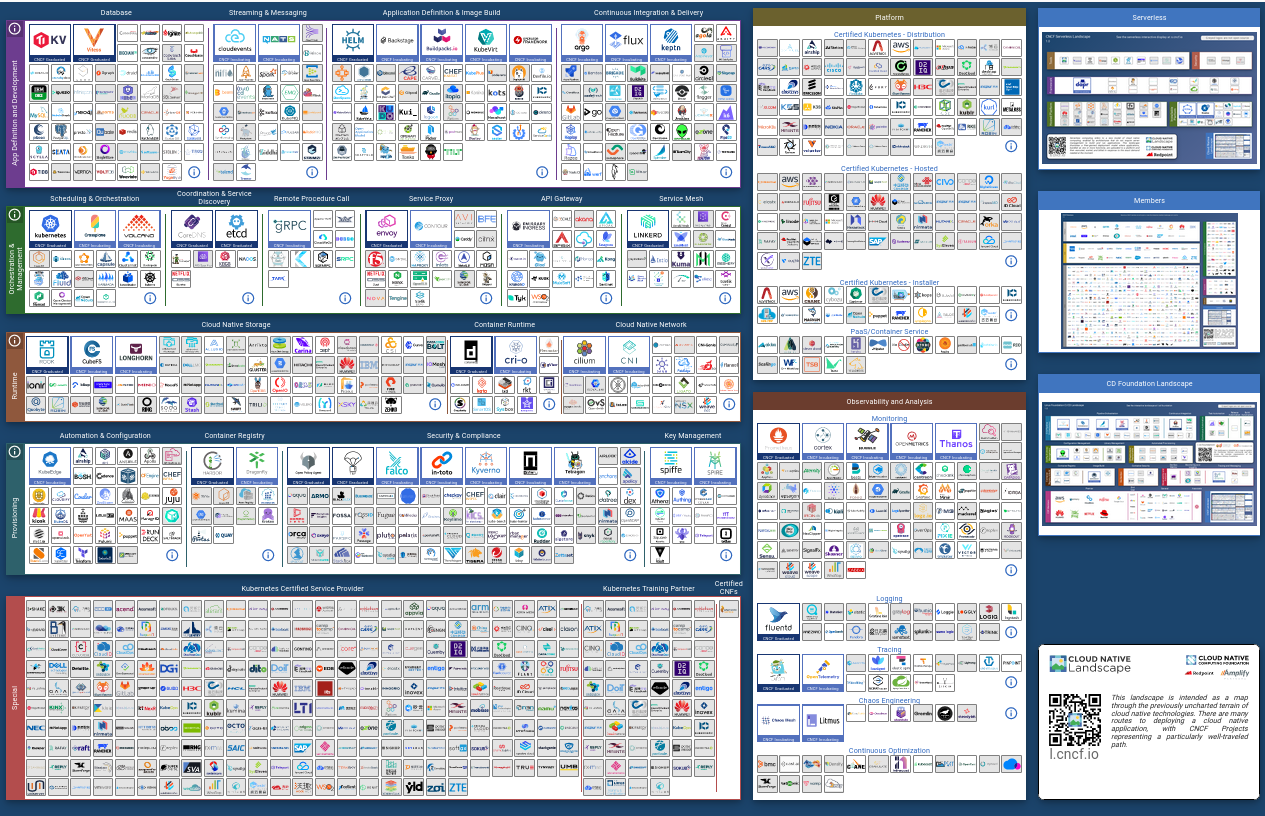
\includegraphics[scale=0.35]{landscape-cncf}
\caption{Landscape CNCF}
\end{figure}

\newpage

\section{Les enjeux et les controverses}

Dans cette section, nous allons dans un premier temps voir les enjeux et les controverses économiques du DevOps, dans un second temps les enjeux et les controverses stratégiques dans le DevOps.

\subsection{Économiques}

En terme économique, nous avons un peu évoqué le sujet mais le DevSecOps permet d'être plus efficace et rapide dans ses cycles de développement, d'assurer une meilleur sécurité et stabilité du produit, et donc par conséquent avoir des enjeux économiques importants au sein des entreprises.

A contrario, cela peut représenter en frein et des pertes économiques, car le DevOps est avant tout une philosophie. 
En effet, pour que cela fonctionne il y a certaines bonnes pratiques à mettre en place, surtout au niveau organisationnel, fonctionner de façon Agile. \\
Par exemple, une des bonnes pratiques de la méthode Agile et quand on se lance dans un projet de logiciel, on fait des rush d'un semaine. Chaque fin de semaine on fait un débrife avec le client, il y a un échange avec d'éventuelles ajustement à faire. \\
Si l'entreprise cliente ne prend pas au sérieux ce rituel, l'entreprise développeuse peut alors perdre du temps et de l'argent.
Ce problème d'adoption de manière de fonctionner peut créer des déséquilibres organisationnelles et engendrer des pertes.

\subsection{Stratégiques}

En terme stratégique, le DevSecOps reste un point central dans l'avenir et le futur développement des entreprises du domaine.
En effet, on peut voir que beaucoup d'entreprises recrutent dans ce domaine, sur LinkedIn les recruteurs et chasseurs de têtes on énormément d'offres pour les personnes du métier. \\

A contrario, il ne faut pas tomber non plus dans le "buzzword", beaucoup d'entreprise parle plus d'un métier avant la culture. On peut remarquer sur le marché des offres d'emploies qui se disent DevOps alors qu'elles le sont juste en apparence.


\chapter{Conclusion}

Pour conclure, la méthode de veille choisie est fait en fonction de mon sujet et de mon besoin d'avoir des informations constantes sur les mises à jours et les évolutions à venir. Je n'aurai pas fait le même type de veille dans une autre situation ou mes choix auraient été différent.
Par exemple, l'outil de flux RSS m'a particulièrement bien aidé car je dois surveiller beaucoup de ressources et de liens différents ce qui est peut être rapidement fastidieux voir en oublier et engendrer des failles de sécurité sur le réseau ou dans les applications. \\

Cette veille m'a permis d'en apprendre plus sur mon cœur de métier, sur son origine mais aussi sur son présent et avenir. Cela m'a appris que cette méthode / culture avait ces limites. Mais ça m'a aussi conforté dans l'idée le DevOps (DevSecOps) est un métier pleins d'avenir et très intéressant. \\

C'est un travail que je vais continuer à l'avenir car elle me permet de monter en compétences sur divers sujets et d'en apprendre plus, cela m'a aussi montré que quand on s'intéresse sur un sujet faire venir l'information à nous peut être très agréable et nous permet d'avoir une analyse poussé sur les tendances à venir.



\chapter{Bibliographie}

\begin{itemize}
\item Cloud Native Computing Foundation, Wikipedia
\item Landscape CNCF, https://landscape.cncf.io/
\item Manifesto for Agile Software Development, https://agilemanifesto.org/, 2001
\item Professionnal DevOps, DevOps vs DevSecOps, https://www.professional-devops.com/images/devops-vs-devsecops.png
\item The Phoenix Project: A Novel about IT, DevOps, and Helping Your Business Win Paperback – Illustrated, February 27, 2018
\end{itemize}



\newpage

\listoffigures

\end{document}
